\section{开发实验：从基线到失效案例}
本节记录阶段 1--3 的实际开发证据。训练、调参和后续边界角点都属于开发数据，不承担最终独立评价的角色。图表由已保存的数值文件重绘；图像生成不计为新的 Moonshine 实验。

\subsection{配置与求解器校验}
\begin{table}[htbp]
\centering
\caption{固定 POD 开发实验配置}
\label{tab:development-config}
\small
\begin{tabular}{lp{0.66\linewidth}}
\toprule
项目 & 配置 \\
\midrule
主网格 & $24\times24$ 个单元，576 个未知量；积分热量方程 \\
参数与采样 & 四个 $h_s\in[0.2,5]$；每个分量在对数尺度均匀采样 \\
训练集 & 24 个参数；NumPy \texttt{default\_rng} 种子 20261025 \\
调参集 & 12 个参数；种子 20261026，与训练参数无重合 \\
快照与候选秩 & 只用训练解，不作中心化；$r\in\{1,2,4,8,12,24\}$ \\
选秩规则 & 选择调参最大场误差不超过 $\tau=10^{-3}$ 的最小候选秩 \\
失效开发集 & 保持所选秩不变，追加 $\{0.2,5\}^4$ 的 16 个角点 \\
数值环境 & Python 3.12.14，NumPy 2.3.5，SciPy 1.18.1 \\
\bottomrule
\end{tabular}
\end{table}

Moonshine 生成的基础校验程序实际运行后，34 项检查全部通过，覆盖手算小矩阵、单单元温度、对称性、热源总量、非负温升、残差、热量守恒和常温平衡。单次该校验包含 7 次线性求解；重复执行不能当作新增的 34 种性质。四组主网格案例的最大相对残差为 $1.1841\times10^{-13}$，最大相对热量不平衡为 $6.2450\times10^{-15}$。单单元 $h_s=2$ 的手算解 $T=0.03$ 也得到复现。

外部独立程序用 Kronecker 结构重新组装了 84 组矩阵与源向量，而非仅调用同一装配代码重复检查。它还使用不同于项目矩形源的光滑制造解，在 $n=8,16,32,64$ 上观测到误差阶约 $1.980,1.979,1.989$。这支持该制造案例的收敛表现，不是原不连续热源下任意网格误差阶的证明，也不计为 Moonshine 自主运行成果。

\subsection{固定 POD 能拟合调参数据，但不是全域保证}
Moonshine 为 36 个训练和调参参数执行完整求解，并对六个候选秩共执行 216 次 ROM 计算。表~\ref{tab:rank-errors} 给出 12 个调参案例的最大场误差，$r=8$ 是首个满足既定规则的候选。图~\ref{fig:development-rank} 同时显示训练与调参误差；秩 24 在训练数据上的近机器精度拟合不能替代其他参数的验证。

\begin{table}[htbp]
\centering
\caption{六个候选秩的调参最大场误差}
\label{tab:rank-errors}
\small
\begin{tabular}{rrrrrrr}
\toprule
$r$ & 1 & 2 & 4 & 8 & 12 & 24 \\
\midrule
$\max e_\infty$ & $1.7299\!\times\!10^{-2}$ & $1.2057\!\times\!10^{-2}$ & $8.2183\!\times\!10^{-3}$ & $3.8407\!\times\!10^{-4}$ & $2.9648\!\times\!10^{-5}$ & $5.3270\!\times\!10^{-8}$ \\
达到 $\tau$ & 否 & 否 & 否 & 是 & 是 & 是 \\
\bottomrule
\end{tabular}
\end{table}

\begin{figure}[htbp]
\centering
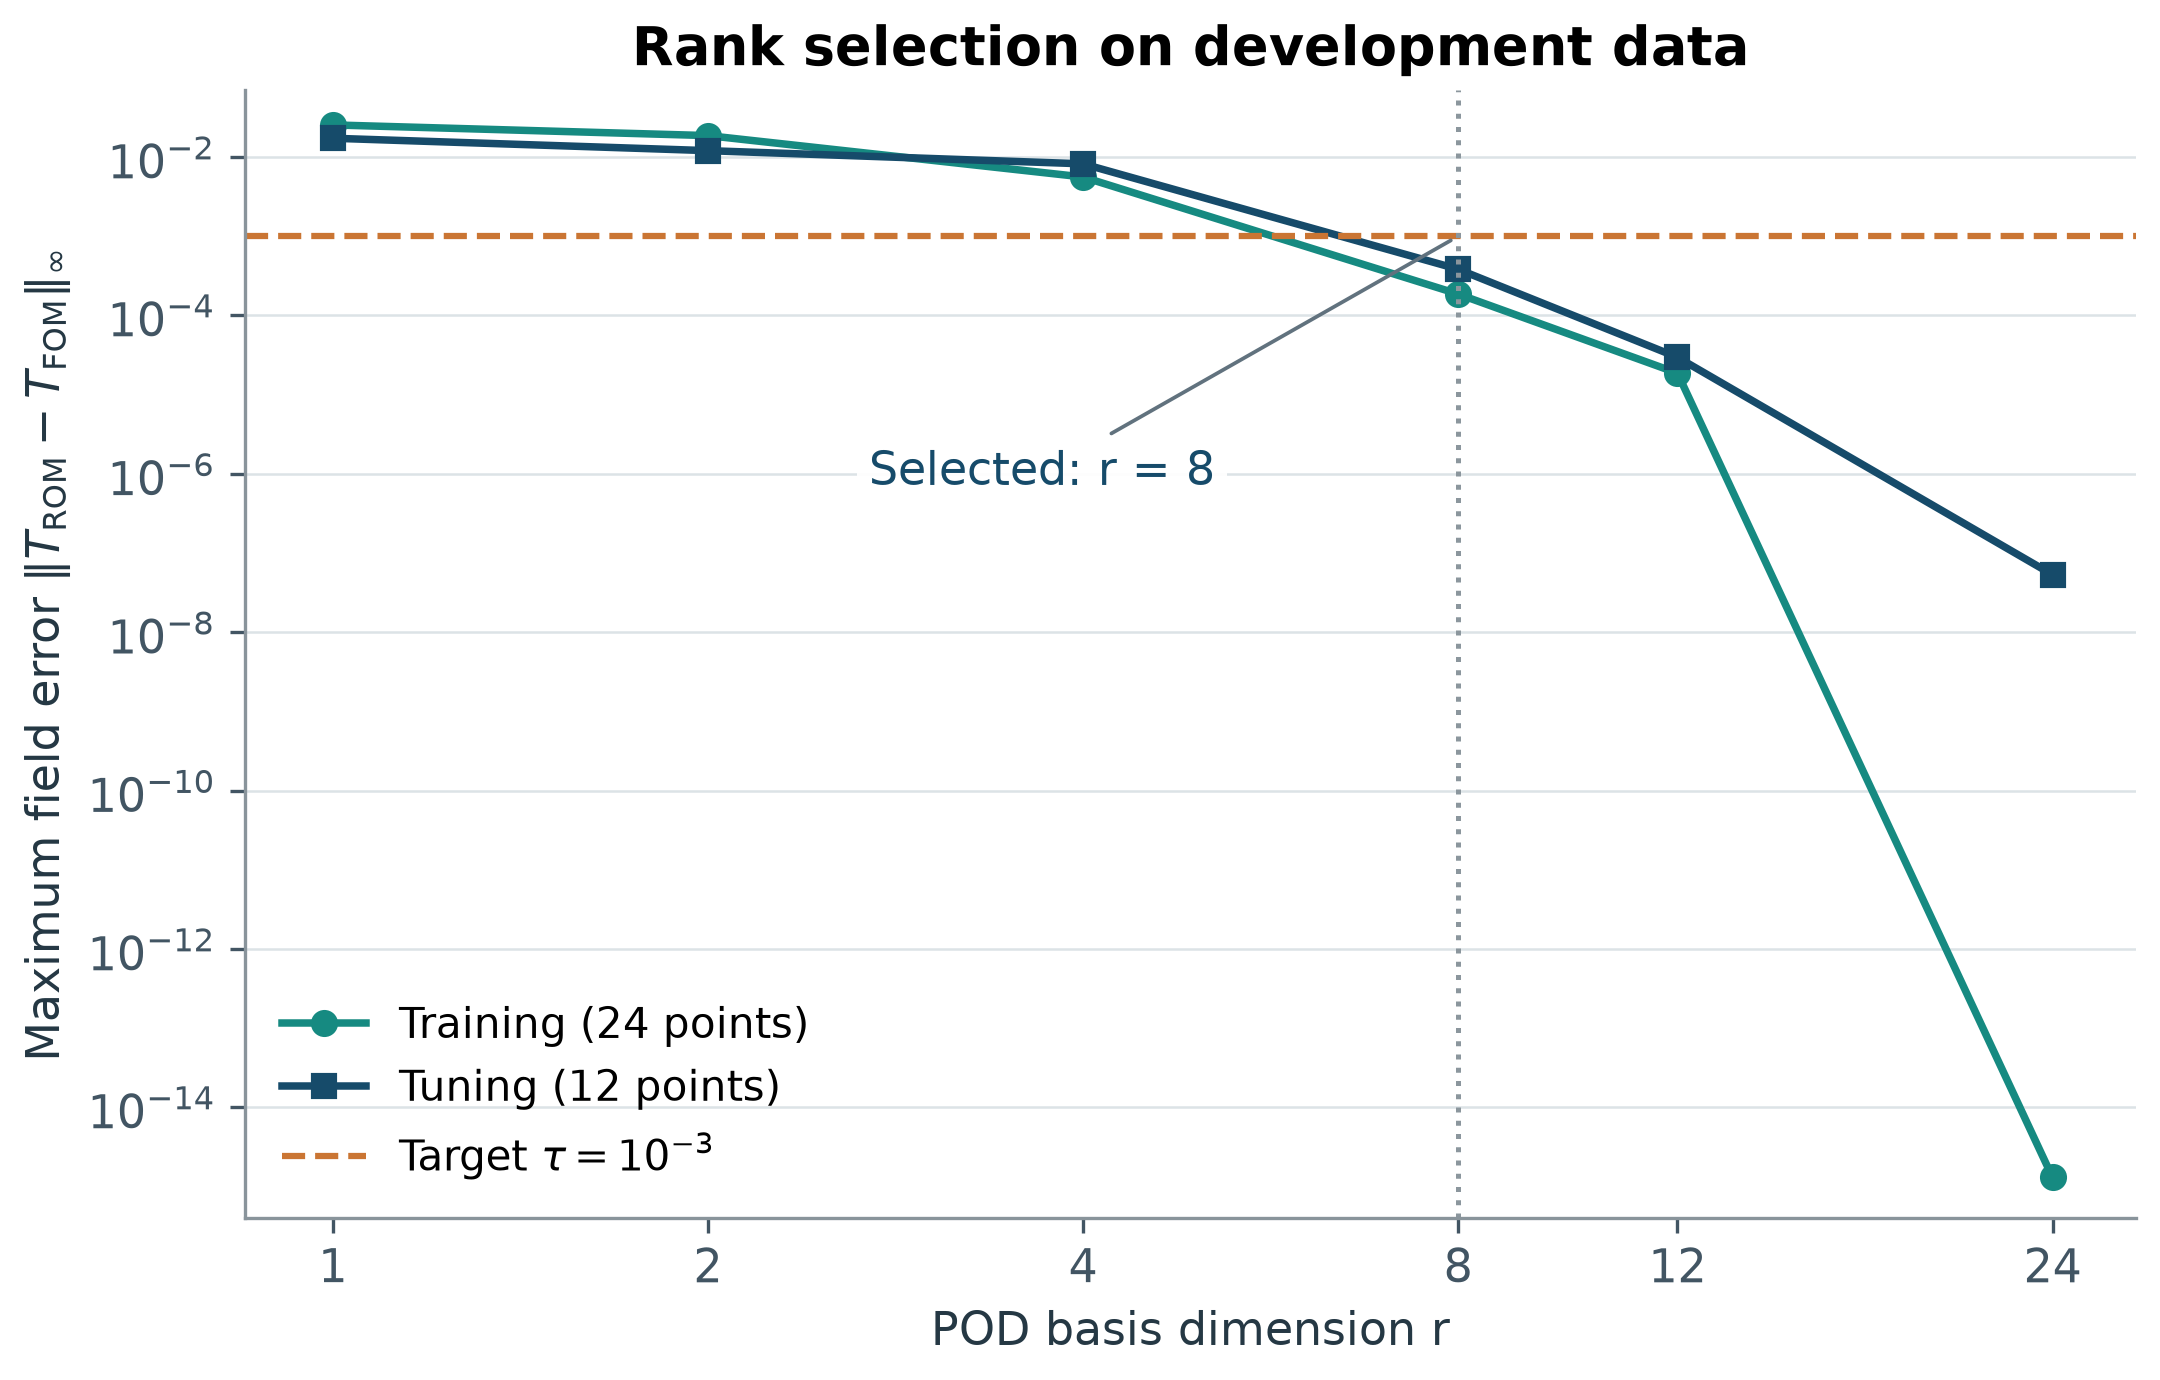
\includegraphics[width=0.78\linewidth,height=72mm,keepaspectratio]{figures/development_rank_curve.png}
\caption{开发数据上的选秩曲线；虚线为场误差目标 $10^{-3}$。}
\label{fig:development-rank}
\end{figure}

保持 $r=8$ 不变后，16 个边界角点中有 2 个\emph{场误差}超标：$\mu=(0.2,0.2,0.2,0.2)$ 的 $e_\infty=3.979763\times10^{-3}$，$\mu=(5,5,5,5)$ 的 $e_\infty=1.408608\times10^{-3}$。这两个点对应的热点值误差分别为 $4.033596\times10^{-4}$ 和 $2.081134\times10^{-4}$，均低于 $10^{-3}$；因此结论是场精度失效，不能改称热点值超标。最坏场误差案例见图~\ref{fig:development-fields}，误差较大区域与最高温位置并不一致。

\begin{figure}[htbp]
\centering
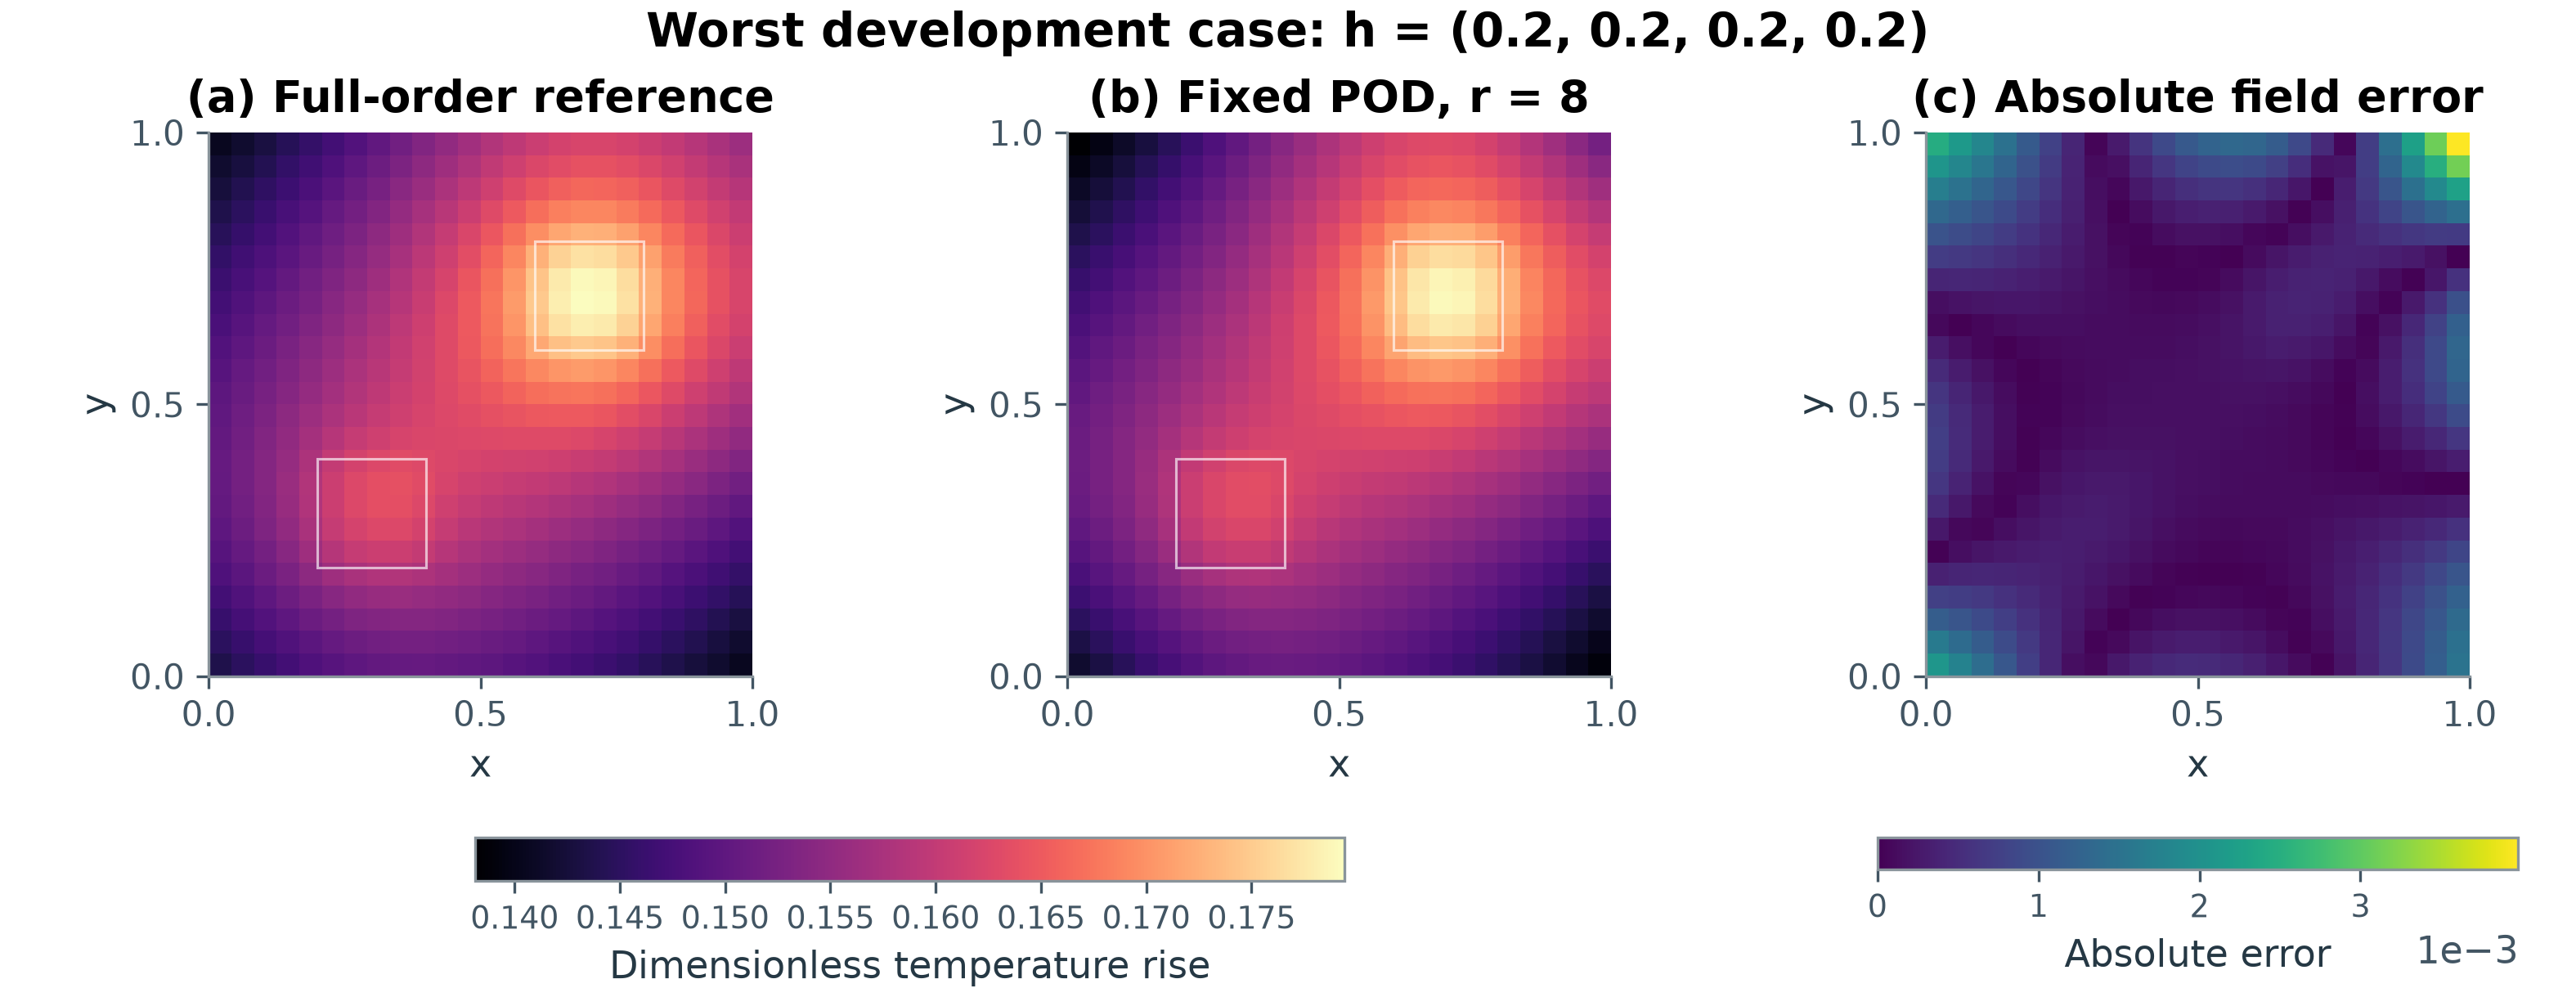
\includegraphics[width=\linewidth,height=64mm,keepaspectratio]{figures/development_worst_fields.png}
\caption{最坏开发案例的完整温度场、固定 POD 与逐点绝对误差。}
\label{fig:development-fields}
\end{figure}

\clearpage
\subsection{屏障覆盖误差，但预警明显保守}
阶段 3 复用 12 个调参案例，另执行 16 次 FOM 和 16 次 ROM，形成 28 个开发案例；没有在本阶段更新基。使用 $\eta>\tau$ 作为候选触发规则时，28 个案例都会触发，其中 2 个确实存在场误差超标，另外 26 个原近似已达到场误差目标。本组案例没有漏警，但不能据此推断任意浮点计算均无漏警。

效能比定义为 $\eta/e_\infty$。这 28 个案例的效能比范围为 $330.329$ 至 $734.112$，中位数为 $529.804$。最坏场误差点的 $\eta=1.417555$，约为实际误差的 $356.191$ 倍。图~\ref{fig:development-indicator} 表明，该界在当前样本上能覆盖误差，却可能引发大量额外完整求解。安全性、保守性和成本是需要同时研究的三个目标，不能只以覆盖误差宣称方法有效。

\begin{figure}[htbp]
\centering
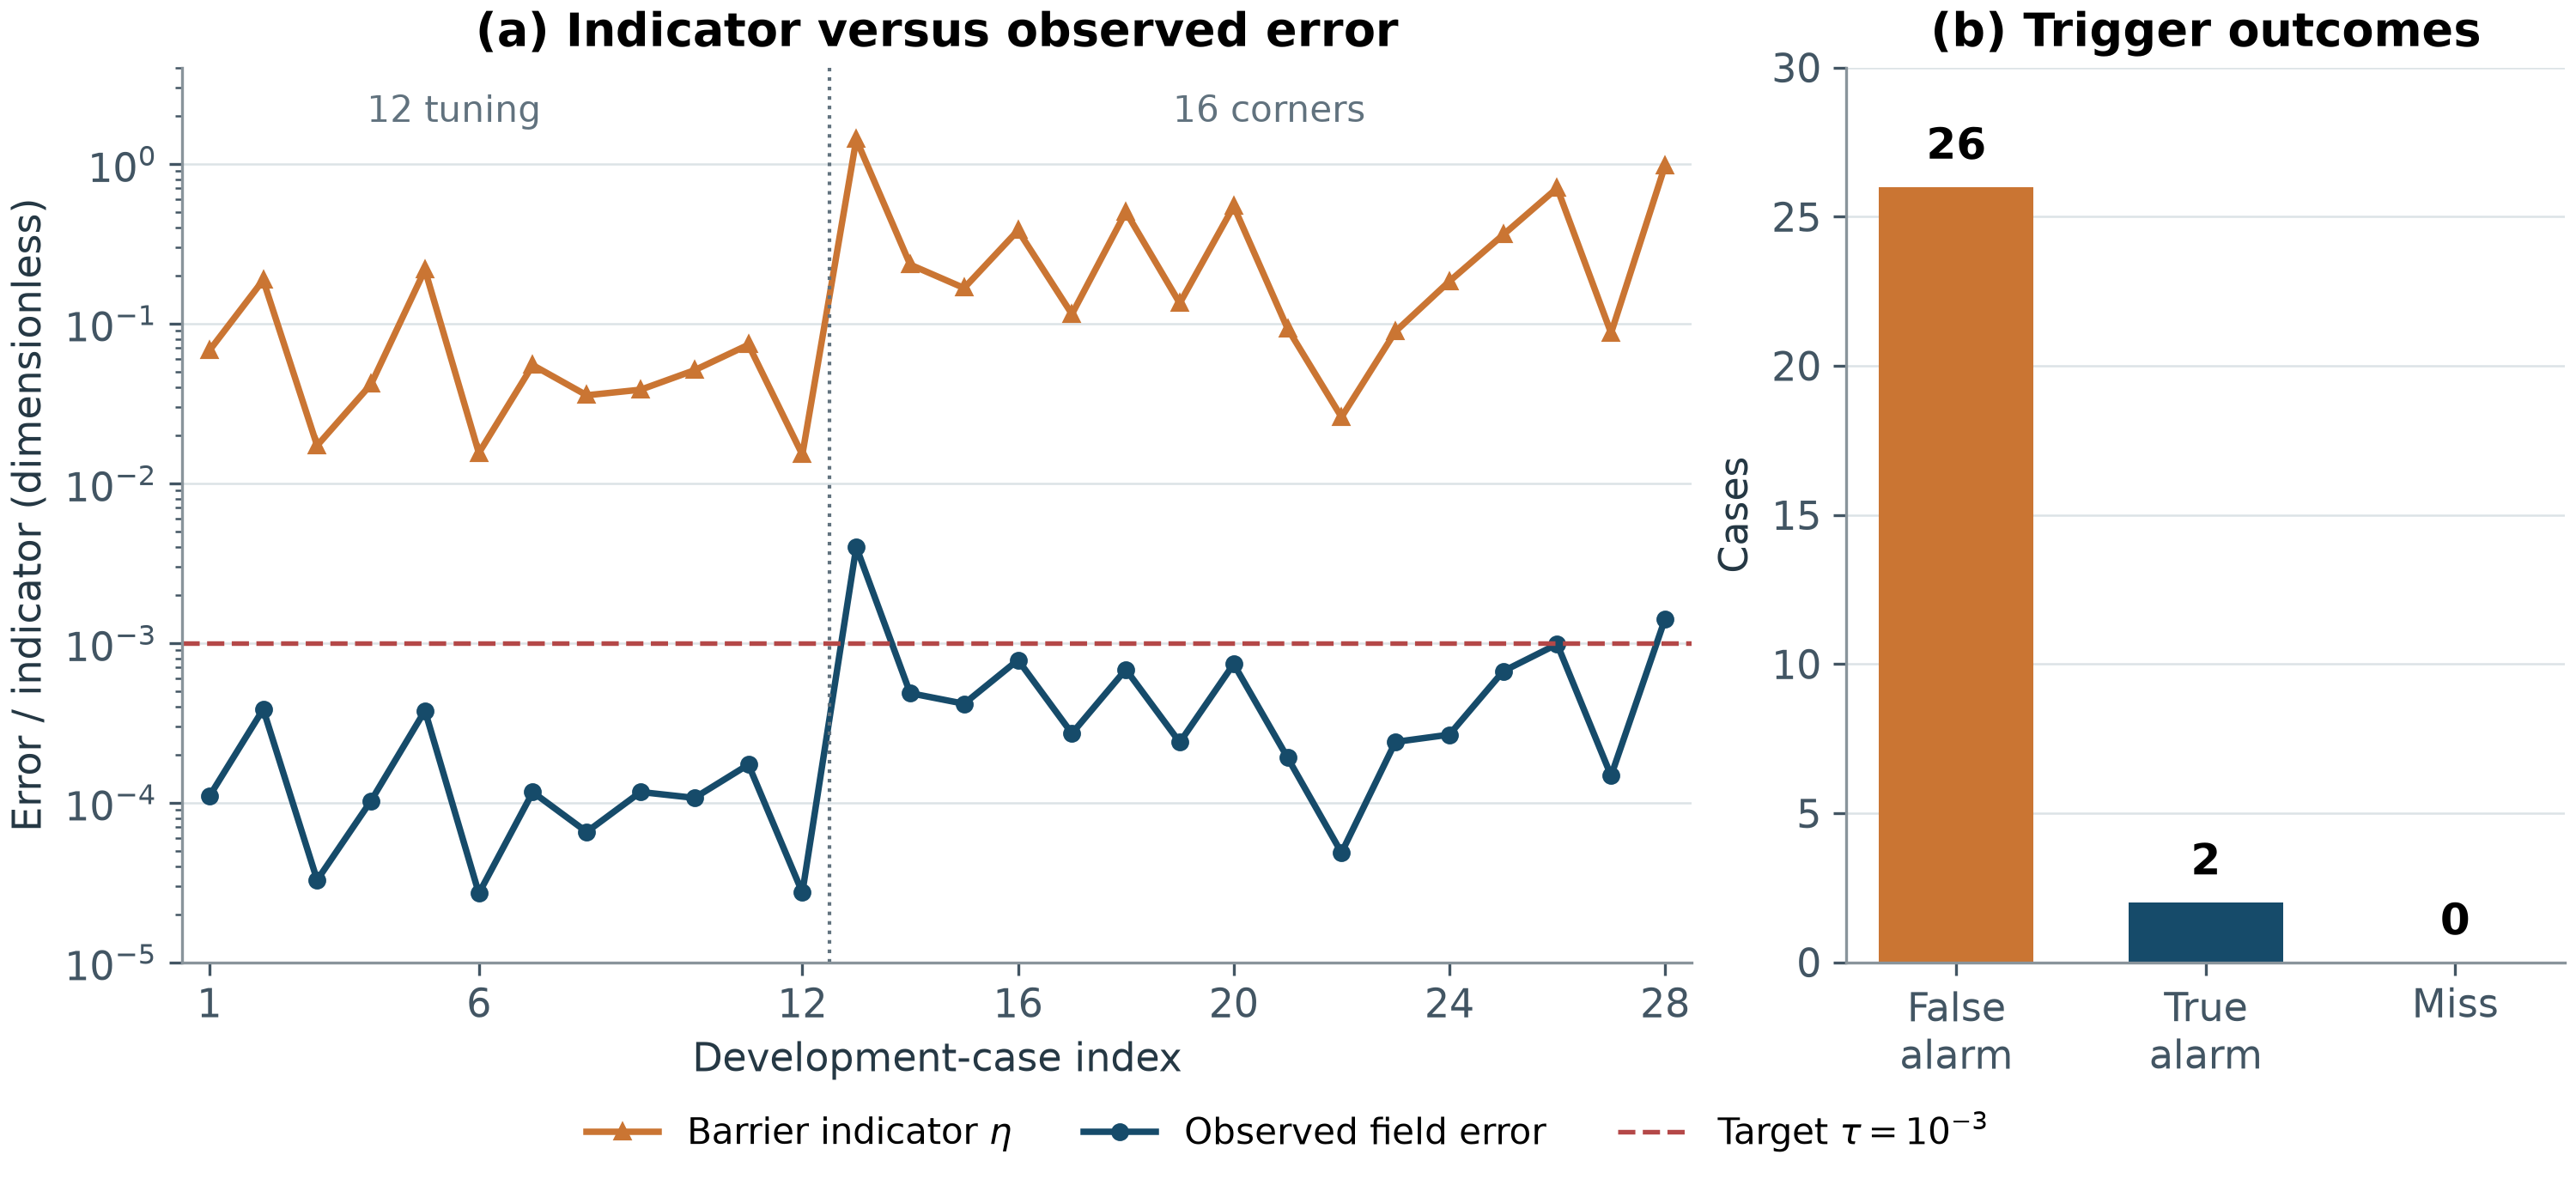
\includegraphics[width=\linewidth,height=75mm,keepaspectratio]{figures/development_indicator_failures.png}
\caption{28 个开发案例的屏障指标与实测场误差；右图按回退前误差统计候选触发。}
\label{fig:development-indicator}
\end{figure}

Moonshine 还以 \texttt{Fraction} 对 $n=1,2,3,4$ 的各 16 个参数角点作精确算术核对，共 64 组、480 个单元，均满足解析屏障不等式。普通双精度检查的最小 $(Az)_P$ 为 $0.9999999999995453$，与精确界的差异处于舍入量级；报告据此保留浮点评估与严格认证之间的区别。

\subsection{加入离线成本后，短批量尚未取得总体加速}
基线开发实现对每个参数重新装配完整矩阵，再投影、求解和重构。其 12 个调参查询的时间分解见表~\ref{tab:development-cost}。所选秩的在线时间比为
\[
 \frac{t_{\mathrm{FOM},12}}{t_{\mathrm{ROM,online},12}}
 =\frac{0.0241535}{0.0138724}\approx1.741.
\]
若按“训练快照、SVD、所选秩的 12 次查询”的部署成本口径，将一次离线成本完整计入，则
\[
 \frac{t_{\mathrm{FOM},12}}
 {t_{\mathrm{snapshot}}+t_{\mathrm{SVD}}+t_{\mathrm{ROM,online},12}}
 =\frac{0.0241535}{0.0677765}\approx0.356.
\]
后一比值小于 1，表示这个短批量下的直接完整求解更省时。不能把 $1.741$ 写成含离线成本的总加速倍数。

\begin{table}[htbp]
\centering
\caption{12 个调参查询的开发阶段时间分解（秒）}
\label{tab:development-cost}
\small
\begin{tabular}{lr}
\toprule
项目 & 实测时间 \\
\midrule
24 个训练快照的离线计算 & 0.0504288 \\
SVD 建基 & 0.0034753 \\
所选 $r=8$ 的 12 次 ROM 在线计算 & 0.0138724 \\
上述离线与在线之和 & 0.0677765 \\
12 次 FOM 组装与求解 & 0.0241535 \\
\bottomrule
\end{tabular}
\end{table}

这些时间来自单次开发观测，存在计时噪声，而且 ROM 在线计时含残差评估，FOM 对照未含另外记录的残差时间，故尚不是统一输出服务下的最终性能基准。上述部署成本也不包括全部选秩搜索、调参与文件保存等研究开销；这些开销保存在原始记录中，没有被宣称为零。开发结果提出了后续比较的具体要求：复用组装结构、设置快速 FOM 对照、统一计时边界，并检验不同查询批量下离线成本能否摊销。

\subsection{外部复算与证据对应}
三份外部复核分别完成 84 组矩阵与源装配对照、36 次 FOM 与 216 次 ROM 复算，以及全部 28 个失效开发案例的 FOM/ROM 复算。基线复算的最大场数组差不超过 $4.025\times10^{-16}$；失效分析的场误差指标差不超过 $5.552\times10^{-17}$，效能比与 $28/2/26$ 触发统计均得到复现。原生的 64 组有理数检查也与外部精确计算一致。以上次数与 Moonshine 原生执行分别记账，不能相加后声称全部由同一智能体自主完成。

数值来源为 \texttt{workspace/results/01\_model.json}、\texttt{02\_baseline.json} 和 \texttt{03\_failure.json}；外部复核依据为 \texttt{independent\_review/stage01\_crosscheck.json}、\texttt{stage02\_crosscheck.json}、\texttt{stage03\_crosscheck.json}。审核状态以原版事件记录为准：早期产物中的“待审核”字段保留其生成时状态，不用事后修改覆盖失败或未定记录。
